
\documentclass[a4paper]{article}
\author{Oscar Emil Sommer}
\input{../preamble}
\input{../macros}

\fancyhead[L]{\textbf{Matrix product states}}


\begin{document}
\section{Lecture 1}
When investigating \emph{many-body quantum systems}, we generally want statistical properties,
even as our models are too complicated to solve exactly.

\begin{example}[Spin chain]
    A system of $L$ spins has a Hilbert space
    $\{\ket{\up},\ket{\down}\}^{\otimes L} $ 
    with  dimension $2^L$ making exact
    numerical calculations completely infeasible for $L\gtrsim 30$
    \begin{center}
    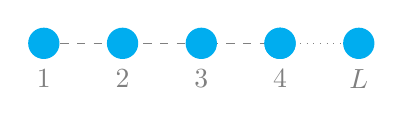
\begin{tikzpicture}
        \tikzset{bead/.style={circle,fill=cyan,inner sep=4pt}}
        \draw[dashed, gray] node[bead,label=below:$1$]{}(0,0)
            \foreach \spin in {2,...,4}
                { -- ++(1,0) node[bead,label=below:$\spin$]{}}
                edge[dotted] ++(1,0) node[bead]{} ++(1,0)
                node[bead,label=below:$L$]{};
    \end{tikzpicture}
    \end{center}
    
\end{example}
Instead we must change our mindset from finding information about all of the
states, and instead focus only on the relevant sectors. For most purposes the
states we are interested are near the \emph{ground state} or \emph{thermal
states}.  Hence we want a method to calculate states in these sectors, which is
where the matrix product state (MPS) method comes into play.\\
\begin{remark}[MPS (PEPS/TNS) methods] Key things to think about are
    \mbox{}
\begin{itemize}
    \item Sysems dimension is usually 1D (or 2D)
    \item Works for Bosons, fermions, spins
    \item Works best for `low' entanglement states, which is quantified later.
    \item There is primarily a possibility of finding ground state and low excited states
    \item It is possible to find time evolution of both closed and open systems
    \item The method works with finite temperature states
\end{itemize}
\end{remark}



\subsection{Idea of DMRG/MPS (Variational method)}
The matrix product state method is a variational method which relies heavily on
Singular value decompositions(SVD) and the Schmidt decomposition.
\begin{method}[Singular Value decomposition]
    Any rectangular matrix $A$ of dimensions $(m\times n)$ can be decomposed as 
\[
A=USV^\dagger,
\]
where the matrices $U,S,V^\dagger$ are matrices with the below properties
\begin{description}
    \item[$U\,\,\,$:] A $\left(m\times\mathrm{min}(m,n)\right)$ matrix with $U^\dagger U=I$
    \item[$S\,\,\,$:] A $\left(\mathrm{min}(m,n)\times\mathrm{min}(m,n)\right)$ diagonal matrix with
            $S_{\alpha\alpha}=\sqrt{\lambda_\alpha}\geq0$
    \item[$V^\dagger$:] A $\left(\mathrm{min}(m,n)\times n\right)$ matrix with $V^\dagger V=I$
\end{description}
The rank of $S$ will turn out to be especially important and so in general we
will denote $r=\text{rank of $S$}$.
\end{method}
\begin{method}[Schmidt decomposition]
    Using SVD we can decompose a general element of a product space
    $\mathcal{H}_A\otimes \mathcal{H}_B$ from a double sum over tensor products
    of basis elements to a single sum over an orthonormal schmidt basis as follows
\begin{align*}
\ket{\psi}&=\sum_{ij}\psi_{ij}\ket{i}_A\ket{j}_B\\
&= \sum_{ij\alpha}U_{i\alpha}\sqrt{\lambda_\alpha} V_{j\alpha}^*\ket{i}_A\ket{j}_B\\
&=\sum_{\alpha=1}^r \sqrt{\lambda_\alpha}\left(\sum_i U_{i\alpha}\ket{i}_A\right)\left(\sum_j
V_{j\alpha}^* \ket{j}_B\right)\\
&=\sum_{\alpha=1}^{r}\sqrt{\lambda_\alpha}\ket{\alpha}_A\ket{\alpha}_B\tag{$\star$}\label{eq:schmidtdecomp}
\end{align*}
\end{method}
The Schmidt decomposition is exact and the coefficients $\lambda_\alpha$ tell us very useful
information about what happens if we trace out one of the two subsystems. It
also provides the minimal number $r$ of coefficients by which we may describe
$\ket{\psi}$ using a product basis. 

The point of matrix product states is now to find a way of implementing
a variational technique for the  states $\ket{\tilde{\psi}}$
which takes the form of \eqref{eq:schmidtdecomp} with only $D\leq r$ terms. For
given $D$ we may vary the basis and coefficients to minimise
$||\ket{\tilde{\psi}}-\ket{\psi}||$.
Without loss of generality we may order the coefficients $\lambda_1\geq
\lambda_2\geq\dots \geq \lambda_r$, which allows us to calculate the minimal
distance
\[ 
\left\lVert\ket{\tilde{\psi}}-\ket{\psi}\right\rVert^2=1-\sum_{\alpha=1}^D \lambda_\alpha.
\]
It is therefore self-evident that this is good approximation if $\lambda_\alpha$ decay quickly.

\subsection{Quantifying validity of approximation}
By thinking of our total system as consisting of two subsystems, and tracing out
one of them we can illuminate the meaning of the coefficients.
\begin{center}
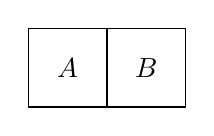
\begin{tikzpicture}
    \draw (0,0) -- (-1,0) -- (-1,1) -- (0,1) -- (0,0);
    \draw (0,0) -- (1,0) -- (1,1) --(0,1) -- (0,0);
    \draw (-0.5,0.5) node[] (){$A$} (0.5,0.5) node[](){$B$};
\end{tikzpicture}
\end{center}
Suppose we are in a pure state of the total system so that
$\rho=\ketbra{\psi}{\psi}$. The reduced density matrices for the subsystems may
be found by tracing out the other part of the Hilbert space 
\begin{align*}
\rho_A&=\Tr_B \rho,\\
\rho_B&=\Tr_A \rho.
\end{align*}
The coefficients $\lambda_\alpha$ are therefore the eigenvalues of the reduced density matrices.
A measure of how mixed the state is the von-Neumann entropy
\[S= - \Tr \rho_A\ln \rho_A=-\sum_\alpha \lambda_\alpha \ln \lambda_\alpha,\]
which is small when $\lambda_\alpha$ decay fast, and maximal when they are all
equal. Hence the approximation is good if $S$ is small.
\begin{remark}
From this we may conclude that MPS methods approximates the true state well for
low entropy states. An equivalent way of viewing these are as states with a low
amount of entanglement \emph{between the subsystems}\footnote{Ask lecturer to
clarify that it is the entanglement between two subsystems which is small}
\end{remark}
\begin{remark}
Some general theorems about the growth of entropy as system size increases are
known
\begin{itemize}
    \item  Ground state of 1D gapped system with short range interaction $S\to
    \mathrm{const}$ as $L\to \infty$. Hence we only require our approximate
    state to have rank $D\sim 2^\mathrm{const}$ indepedent of system size.\footnote{Shouldn't the
    ground state be a pure state? Ask follow up, if means ground state of
combined system $A+B$.}
    \item  Ground state of 1D critical system $S\to R \ln L+\mathrm{const}$ need $D\sim
        L^R$, which is polynomial in $L$, and therefore much more tractable than
        the exponential growth we see in the dimension of the full Hilbert
        space. 
\end{itemize}
\end{remark}
\subsection{What are MPS?}
So far we have no idea how we are going to implement our minimisation technique,
or where the matrix product states come into play. Any $\ket{\psi}\in
\mathcal{H}^{\otimes
L}$ state can be
decomposed into a so-called MPS by essentially unfolding the coefficients of
into a product of matrices. Let 
\[
\ket{\psi}=\sum_{\sigma_1\cdots\sigma_L} C_{\sigma_1,\dots,\sigma_L}\ket{\sigma_A}\otimes\cdots\otimes\ket{\sigma_L}
\]
be a representation of any given state. Now define a matrix $\psi$ of dim $d\times
d^{L-1}$ where $d=\mathrm{dim}\mathcal{H}$ by the relation
\[\psi_{\sigma_1,(\sigma_2,\dots,\sigma_L)}=C_{\sigma_1\sigma_2\dots\sigma_L}\]
Clearly we can do SVDs iteratively on $\psi$
\begin{align*}
    \psi_{\sigma_1,(\sigma_2,\dots\sigma_L)}&=\sum_{a_1=1}^{r_1} U_{\sigma_1,a_1}
S_{a_1,a_1} (V^\dagger)_{a_1,(\sigma_2,\dots,\sigma_L)}\\
&=\sum_{a_1=1}^{r_1} A^{\sigma_1}_{a_1} C_{a_1,\sigma_2,\dots \sigma_L}\\
&=\sum_{a_1=1}^{r_1}\sum_{a_2}^{r_2} A_{a_1}^{\sigma_1}
U_{(a_1,\sigma_2),a_2} S_{a_2a_2}
(V^{\dagger})_{a_2,(\sigma_3\dots\sigma_L)}\\
&=\sum_{a_1,a_2}
A_{a_1}^{\sigma_1}A_{a_1a_2}^{\sigma_2}\psi_{(a_2,\sigma_3)(\sigma_4\cdots)}\\
&=\sum_{a_1\dots a_{L-1}} A^{\sigma_1}_{a_1} A^{\sigma_2}_{a_1a2}\cdots
A_{a_{L-2}a_{L-1}}^{\sigma_{L-1}} A_{a_{L-1}}^{\sigma_L}
\end{align*}
Where we've decomposed the tensor coefficient into a product of matrices of
dimension  $(1\times d)(d\times d^2)\dots (d^{L/2-1} \times d^{L/2})( d^{L/2}
\times d^{L/2 -1})\dots(d\times 1)$. It can be nice to think about what we are
doing in diagrams, by representing a tensor as a square with lines corresponding
to each index. Our matrix product state then is constructed by pulling apart
each of the external indices as



\begin{center}

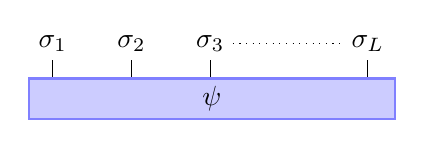
\begin{tikzpicture}[inner sep=1mm]
    \tikzstyle{tensor}=[rectangle,draw=blue!50,fill=blue!20,thick]
    \foreach \i in {1,...,3} {
        \node[tensor] (\i) at (\i, 0) {};

        \node[] (s\i) at (\i, 0.7) {$\sigma_\i$};
        \draw[-] (\i) -- (s\i);
    };

    \draw (3) edge[dashed] (5,0);
    \node[tensor](5)at (5,0){};
    \node (s5) at (5,0.7) {$\sigma_L$};
    \draw[-] (5) -- (s5);

    \draw[dotted] (s3) -- (s5);

    \node[tensor,minimum width=4.65cm] (0) at (3.02, 0) {$\psi$};
\end{tikzpicture}\\
{\large$\Downarrow$}\\
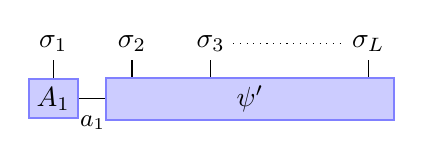
\begin{tikzpicture}[inner sep=1mm]
    \tikzstyle{tensor}=[rectangle,draw=blue!50,fill=blue!20,thick]
    \foreach \i in {1,...,3} {
        \node[tensor] (\i) at (\i, 0) {$A_\i$};

        \node[] (s\i) at (\i, 0.7) {$\sigma_\i$};
        \draw[-] (\i) -- (s\i);
    };

    \draw (3) edge[dashed] (5,0);
    \node[tensor](5)at (5,0){};
    \node (s5) at (5,0.7) {$\sigma_L$};
    \draw[-] (5) -- (s5);

    \draw[dotted] (s3) -- (s5);
    \draw[-] (1) edge[-]node[label=south:\small$a_1$]{} (2);
    \node[tensor,minimum width=3.65cm] (0) at (3.5, 0) {$\psi'$};
\end{tikzpicture}\\
{\Large$\Downarrow$}\\
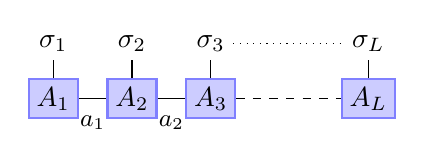
\begin{tikzpicture}[inner sep=1mm]
    \tikzstyle{tensor}=[rectangle,draw=blue!50,fill=blue!20,thick]
    \foreach \i in {1,...,3} {
        \node[tensor] (\i) at (\i, 0) {$A_\i$};
        \node (s\i) at (\i, 0.7) {$\sigma_\i$};
        \draw[-] (\i) -- (s\i);
    };
    \foreach \i in {1,...,2} {
        \pgfmathtruncatemacro{\iplusone}{\i + 1};
    \draw (\i) edge[-] node[label=south:\small$a_\i$]{}(\iplusone);
};

    \draw (3) edge[dashed] (5,0);
    \node[tensor](5)at (5,0){$A_L$};
    \node (s5) at (5,0.7) {$\sigma_L$};
    \draw[-] (5) -- (s5);
    \draw[dotted] (s3) -- (s5);
\end{tikzpicture}
\end{center}
%TODO  Rewatch end 
\section{Lecture 2}
Now the MPS is an exact representation, but given that the matrices grow
exponentially in size in the middle of the chain, it is necessary to approximate
the matrices. This is where the Schmidt decomposition comes in.
\begin{remark}
    We started from the left in our expansion; this is called
    \emph{left-canonical} MPS or \emph{left-normalised}. This means that 
    \[
        \sum_{\sigma_l} {A^{\sigma_l}^\dagger A^{\sigma_l} =I
    \]
    This follows from 
    \begin{align*}
        \sum_{\sigma_l} \left(A^{\sigma_l}^\dagger A^{\sigma_l}\right)_{a_l a'_l}
        &=\sum_{\sigma_l, a_{l-1}} (U^\dagger)_{a_l,a_{l-1}\sigma_l}
            U_{a_{l-1}\sigma_l, a'_l}\\
        &=\delta_{a_l,a'_l}
    \end{align*}
    Equivalently one can begin reshaping from right to get 
    \[
        \ket{\psi}=\sum_{\sigma_1\dots\sigma_l} B^{\sigma_1}\cdots
        B^{\sigma_L}\ket{\sigma_1\dots\sigma_L}
    \]
Which now satisfy $\sum_{\sigma_l} B^{\sigma_l} {B^{\sigma_l}}^\dagger$.
Finally we may do both from left and right, and meet at $l$, so get
\emph{mixed-canonical}, where 
\begin{align*}
    C_{\sigma_1\cdots \sigma_L}&= A^{\sigma_1}\cdots A^{\sigma_l}
    S B^{\sigma_{l+1}}\cdots B^{\sigma_L}
\end{align*}
which essentially gives us a Schmidt decomposition
\begin{align*}
    \ket{\psi}=  \sum_{a_l} S_{a_l,a_l} \ket{a_l}_A\ket{a_l}_B\\
    \ket{a_l}_A&=\sum_{\sigma_1\dots\sigma_l}(A^{\sigma_1}\cdots
    A^{\sigma_l})_{1,a_l}\ket{\sigma_1\dots\sigma_l}\\
    \ket{a_l}_B&= \sum_{\sigma_{l+1}\dots\sigma_L} B^{\sigma_{l+1}}\cdots
    B^{\sigma_L}){a_l,1}\ket{\sigma_{l+1}\dots \sigma_L}
\end{align*}
\end{remark}
Now what we do is cut down the rank of $S$ to a managable number. This
approximation is called \emph{compression}.
A:  is left normalised
B: is right normalised
M: is 

\begin{method}[Compression by SVD]
    Matrix dimension initially $D'$.
    Want to decrease this to dimension $D<D'$.
    \begin{align*}
        \sum_{\sigma_1\dots\sigma_L} A^{\sigma_1}\cdots A^{\sigma_{l-1}}
        M^{\sigma_l} B^{\sigma_{l+1}}\cdots
        B^{\sigma_L}\ket{\sigma_1\dots\sigma_L}
    \end{align*}
    Now use SVD on $M^{\sigma_l}= USV^{\dagger}$ where $S$ is of dim $D'\times
    D'$. Keep only $D$ largest eigenvalues of $S$, to replace $M$ with
    $\tilde{U}\tilde{S}\tilde{V}^\dagger$. Now reshape to $A^{\sigma_l}$, and
    move through $\sigma_l$ iteratively.
\end{method}
\emph{Matrix product operators} (MPO)

\begin{align*}
    O&=\sum_{\sigma,\sigma'} W^{\sigma_1\sigma'_1}\dots W^{\sigma_L \sigma_L'}
    \ketbra{\sigma}{\sigma'}\\
     &=\sum C_{(\sigma_1\dots\sigma_L)(\sigma_1'\dots\sigma_L')}
     \ketbra{\sigma}{\sigma'}
\end{align*}
where we have performed SVD to reshape $(\sigma_l,\sigma'_l)$ extract the sigma indices 
         s1  s2
         |   |
    O = [ ]-[ ]-..
         |   |
         sp1 sp2

Can apply to operator
         \begin{align*}
             O\ket{\psi}&=\sum_{\sigma\sigma'}
             W^{\sigma_1\sigma'_1}M^{\sigma_1'}\dots\ket{\sigma'}
         \end{align*}


Graphical form

 |   |   | 
[ ]-[ ]-[ ]-          | | |
 |   |   |       =>   o=o=o=
 * - * - * -

 \begin{example}[Heisenberg Hamiltonia]
     \[
         H=\sum_i^{L-1} \frac{J}{2}\left( S_i^+ S_{i+1}^- + S^-_i
         S^+_{i+1}+\right) +J^z\sum_{i=1}^{L-1} S^z_i S^z_{i+1} - h\sum_{i=1}^L
         S^z_i
     \]
     This is a $XXZ$ model

     Now convert to MPO

     $W_{b_{l-1}b_l}^{\sigma_l\sigma_l'}\to
     \left(W^{[l]}_{b,b'}\right)_{\sigma_l\sigma_l'}$ a $d\times d$ matrix

     \[
     W^{[i]}=\begin{bmatrix}
     
     \end{bmatrix}
 \end{example}
 Will not describe how to find $W$, but is not hard for standard hamiltonians.
 \subsection{Time evolution with MPS}
Why is it interesting? Recent experimental setups have allowed us to control
time evolution.
Literature: TEBD algorithm G.Vidal PRL 91,147902(2003)
t-DMRG: A Daley et all JStatMech: Theo Exp P04005(2004) 
      : SR white and A Feighah PRL93.076401

Here focus on Trotter-Suzuki decomposition.

Assume XXZ model from before $H=\sum_i h_i$ where $h_i$ only depends on site $i$
and $i+1$.
Want to follow time evolution of state $\ket{\psi_0}$.
Use Schrödinger equation
\[
    i\partial_t\ket{\psi}=H\ket{\psi} \longrightarrow U(t,t+\Delta
    t\ket{\psi(t)}=e^{-i\Delta t H} \ket{\psi(t)}
\]

Want to reach time $t$, discretize to time steps $\Delta t$, so that $t=N\Delta
t$, where $\Delta t$ compared to the energy scale. 
\begin{remark}
    In practice need $\Delta t \lesssim \frac{1}{100 E_\mathrm{char}}$
\end{remark}
Perform Trotter Suzuki decomposition of time evolution operator 

\[
    e^{-i\Delta t H} \simeq \prod_{j\in \text{odd}} e^{-ih_j\Delta t}\prod_{j\in
    \text{even}} e^{-i h_j\Delta t} + \O(\Delta t^2)
\]
error from non-commutitativty of $h_i$ and $h_{i+1}$.
\begin{remark}
    Typically one uses second order 
\[

    e^{-i\Delta t H} \simeq \prod_{j\in \text{odd}} e^{-ih_j\Delta t/2}\prod_{j\in
    \text{even}} e^{-i h_j\Delta t} \prod_{j\in \text{odd}} e^{-ih_j\Delta t/2}
    +\O(\Delta t^3)
\]
\end{remark}
$N$ times gives order of $N\Delta t^3=t \delta t^2$ error
\end{document}
